\documentclass[border=0.2cm]{standalone}

% required packages and libraries
\usepackage{tikz}
\usetikzlibrary{automata, positioning}

\begin{document}

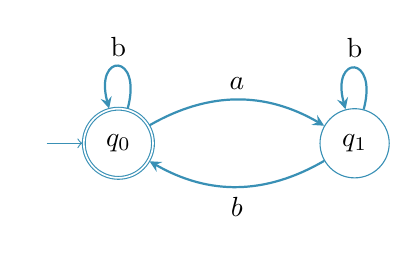
\begin{tikzpicture} [draw=cyan!70!black,
    node distance = 3cm,
    on grid,
    auto,
    every loop/.style={stealth-}]

% State q0
\node (q0) [state,
    initial,
    accepting,
    initial text = {}] {$q_0$};

% State q1
\node (q1) [state,
    right = of q0] {$q_1$};

% Arrows
\path [-stealth, thick]
    (q0) edge[bend left] node {$a$}   (q1)
    (q1) edge[bend left] node {$b$}   (q0)
    (q0) edge [loop above]  node {b}()
    (q1) edge [loop above]  node {b}();
\end{tikzpicture}

\end{document}
